\documentclass[main]{subfiles}

\begin{document}

\section{Empirical Results}\label{sec:results}
In this section, we consider real data examples to compare the performances of different flavors of UACP, with different number of sources and different sizes of the sources. We consider seven different scenarios for the number and size of the data sources, we call them different methods.  We apply these different methods to five real datasets. For each dataset, we split the data into ten folds, where each fold consists of a training set and an independent test set.Then we apply these different methods to all ten folds of each five real datasets. In order to compare the various methods, we look at the two performance measures validity (\ref{eq:validity}) and efficiency (\ref{eq:efficiency}). %All reported results are based on application of different methods to all ten folds of each five real datasets. 

For each dataset we consider the following configurations:

\begin{enumerate}

\item Given a dataset, we split the data into ten folds, where each fold consists of a training set (80\%) and an independent test set (20\%).

\item for each folds we split the training dataset into various number of sources, as follow:
\begin{enumerate}
	\item Single source or pooled data  where training set is considered as a single source.
	\item Equal sized sources: training set is randomly partitioned into equal sized sources and  each partition is considered as a proper training set to model and compute p-values, and then p-values are aggregated for all sources. We mainly consider 2, 4 and 6 equal sized sources. %in three different settings.
	\item Unequal sized sources: training set is randomly partitioned into unequal sized sources and  each partition is considered as a proper training set to model and compute p-values, and then p-values are aggregated for all sources. We mainly consider 2, 4 and 6 unequal sized sources, and we repeat it five times to get five different set of sizes for each source.

\end{enumerate}

\end{enumerate}

Repeat the step 1 and step 2 with five different datasets, and combine the results for each method. Then paiwise compare the validity and efficiency for all methods. %Single source, 2EqualSizedSource, 4EqualSizedSource, 6EqualSizedSource, 2UnequalSizedSource, 4UnequalSizedSource and 6UnequalSizedSource. The details of the datasets used and the results on individual datasets are given in Supplementary Material.%are given in the following, these data have been taken from the UCI Repository of machine learning batabases: ftp://ftp.ics.uci.edu/pub/machine-learning-databases/.


%\subsection{Empirical results on Combined data}
The results for comparing the different methods on combined results, by applying the Wilcoxon signed-rank test on validity and efficiency are shown in Figure \ref{fig:testCombined}. To quantify the difference between various methods the box plots are given in Figure \ref{fig:boxplotCombined}.

\begin{figure}[H]
\centering
\begin{subfigure}{\textwidth}
  \centering
  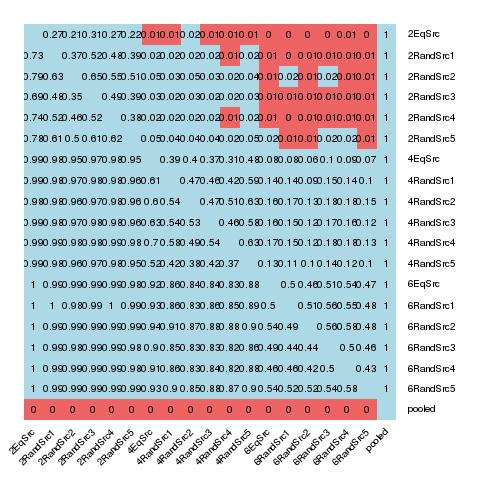
\includegraphics[width=.75\linewidth]{images/heatmapCombined}
%  \caption{Validity}  \label{fig:valCombined}
\end{subfigure}%

\begin{subfigure}{\textwidth}
  \centering
  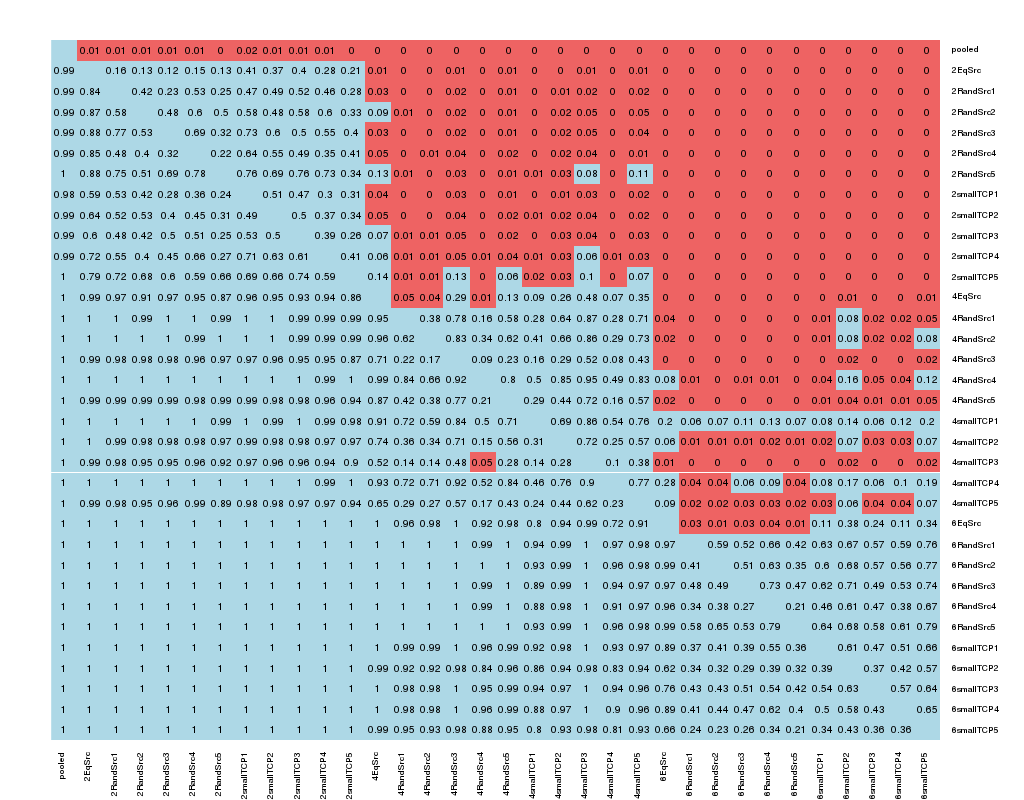
\includegraphics[width=.75\linewidth]{images/heatmapCombined_eff}
  %\caption{Efficiency}  \label{fig:effCombined}
\end{subfigure}%
\caption{Results of Wilcoxon signed-rank tests for two alternative hypotheses relating validity (a) and observed fuzziness (b) with combining all the datasets. The p-values are shown for the methods in the right column having greater values than the methods in the first row. All significant p-values are marked in red. Pooled: Unpartitioned dataset. EqSrc: equally partitioned data sources, RandSrc: randomly partitioned data sources. smallTCP: a single TCP model.} \label{fig:testCombined}
\end{figure}

%Another figure


\begin{figure}[H]
\begin{center}

%\begin{subfigure}{\textwidth}\centering
%  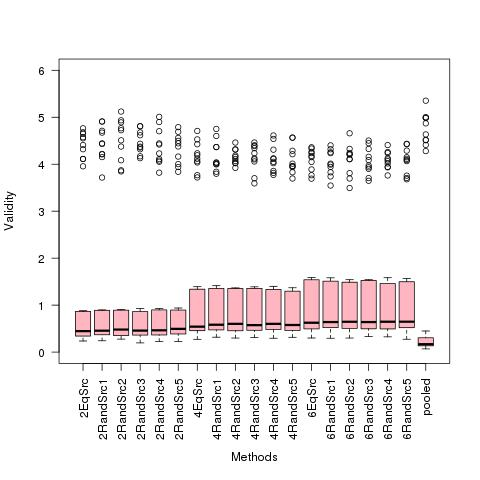
\includegraphics[width=12cm,height=6cm]{images/boxplotCombined}
%  \caption{Validity}  \label{fig:valBC}
%\end{subfigure}%

%\begin{subfigure}{\textwidth} \centering
 
  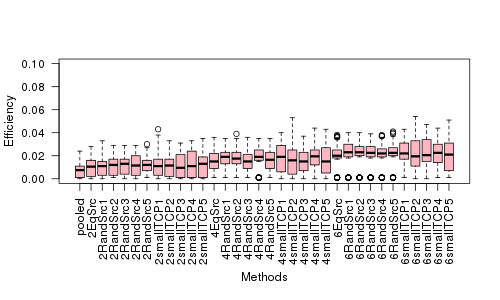
\includegraphics[scale=0.8]{images/boxplotCombined_eff}
 % \caption{Efficiency}  \label{fig:effBC}
%\end{subfigure}%
%\caption{Box plot of validity (a) and observed fuzziness (b) with combined data.}
\caption{Box plot of observed fuzziness for aggregating 0, 2, 4, and 6 non-disclosed data sources. Pooled: Unpartitioned dataset. EqSrc: equally partitioned data sources, RandSrc: randomly partitioned data sources. smallTCP: a single TCP model.}
\label{fig:boxplotCombined}
\end{center}
\end{figure}




\section{Discussions}
The aim of this study was to improve predictions over different data sources without explicitly sharing the data, by aggregating conformal predictions computed at individual locations. In order to do so, we investigated if and how the number of data sources and size of these affect the aggregated efficiency and validity.

Results in Figure~\ref{fig:testCombined} show that pooled is significantly more efficient than all other models, as would be expected, but in absolute numbers the decrease in efficiency is not so large when using an aggregated approach. When comparing uACP with individual smallTCP, we do not see a significant improvement in efficiency using uACP but we observe a reduced variance, consistent with previous work~\cite{Carlsson:2014qr}, when there are 4 or more partitions. We also observe in Figure~\ref{fig:testCombined} that there is no significant difference between 'aggregated equally partitioned' and 'aggregated randomly partitioned', which would make the method generally applicable regardless of the sizes of individual training sets.

%uACP more efficient predictions than individual analyses
%1. To investigate if and how the number of data sources and size of the sources affect the aggregated efficiency and validity

%\subsection{Validity}
Regarding validity, we observe that the pooled model is always valid, as an example see Figure~\ref{fig:pooledCalibrationPlot} for the Spambase dataset. Further, we see that individual small models also all are valid, see Figure~\ref{fig:valIndividual} for randomly partitioned small TCPs for Spambase dataset. Consistent with previous work by Linusson et al~\cite{Linusson:2017dn} and Carlsson et al.~\cite{Carlsson:2014qr}, uACP is less valid overall, see Figure~\ref{fig:valCombined} for randomly partitioned uATCPs for Spambase dataset, but calibration plot shows conservative validity for the significance levels 0 to 0.5 which is the interesting region for predictions. This is a known issue that requires further research; we settle here with the observation that validity does not seem to be a practical problem for uACP in the interesting significance region.

\begin{figure}[H]
\begin{center}
  \begin{subfigure}{.3\textwidth}
  \centering
  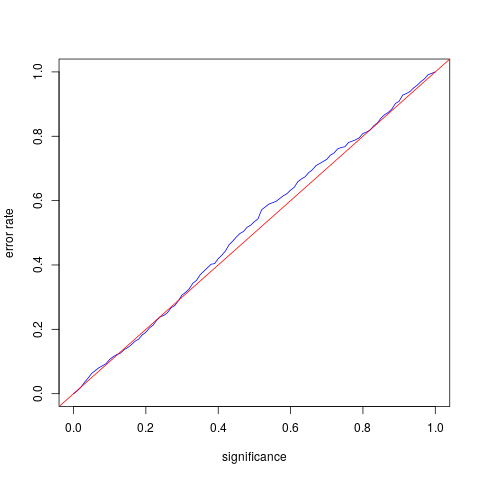
\includegraphics[scale=0.2]{images/pooledCalibrationPlot}
  \caption{pooled} \label{fig:pooledCalibrationPlot}
   \end{subfigure}    
  \begin{subfigure}{.3\textwidth}
  \centering
  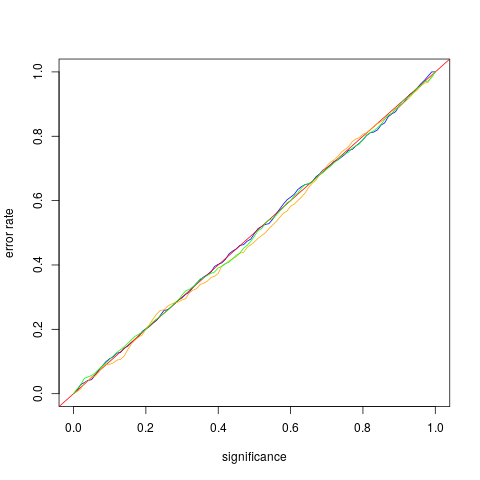
\includegraphics[scale=0.2]{images/eqSourceInd}
  \caption{smallTCPs}\label{fig:valIndividual}
  \end{subfigure}
  \begin{subfigure}{.3\textwidth}
  \centering
  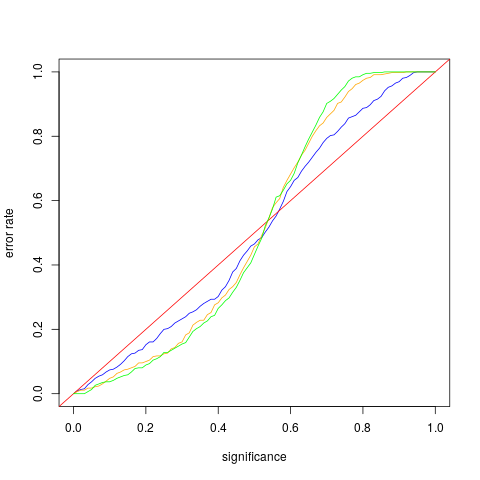
\includegraphics[scale=0.2]{images/eqSourceCombined}
  \caption{uATCPs}\label{fig:valCombined}
  \end{subfigure}
  
 \caption{Calibration plot for various models. a) Calibration plot of TCP for one fold of Spambase dataset. b) Calibration plot of randomly partitioned small TCPs for one fold of  Spambase dataset. Blue, orange and  green line indicate each small TCP from two, four and six source random partitions respectively. c) Calibration plot of uATCPs for one fold of Spambase dataset. Blue, orange and  green line indicate uATCP from two, four and six source random partitions respectively}
 
\end{center}
\end{figure}


%\subsection{Efficiency}
%2. to evaluate how good both aggregated equally partitioned and aggregated randomly partitioned perform when compared to the whole (pooled) data set.


%3. to evaluate if and under what conditions unbalanced aggregated TCP delivers acceptable results when compared to pooled data





\section{Conclusions}
We present a method to aggregate conformal predictions from multiple sources while preserving data privacy. The method is a generalization of the basic conformal prediction framework to handle multiple data sources without disclosing data between the data sources. Due to its low complexity for implementation, we believe the method will be useful for organizations that wish to make predictions over combined data without disclosing data to each other, such as for drug discovery problems when pharmaceutical companies wishes to establish predictive models of drug safety.




\end{document}



